
\subsection{Types}
In C\# gibt es drei Kategorien von Typen. 
\begin{multicols}{2}
\begin{itemize}
	\item Value Types
	\begin{itemize}
		\item Primitive Types (bool, int, char, long \ldots)
		\item Enums
		\item Structs
	\end{itemize}
	\item Pointers
	\item Reference Types
	\begin{itemize}
		\item Class
		\item Interface
		\item Arrays
		\item Delegates
	\end{itemize}
\end{itemize}
\end{multicols}

Unter \textbf{User-defined Types} versteht man Enum, Struct, Class, Interface, Array und Delegate.
Alle \emph{Types} sind kompatibel mit \emph{object}

\subsubsection{Value vs. Reference}
\begin{tabular}{|c|c|c|}
	\hline
	\textbf{Variable of} & \textbf{Values Types}  & \textbf{Reference Types} \\ \hline
	     constrins       &         value          &         referenc         \\ \hline
	     stored on       & stack (or in a object) &           heap           \\ \hline
	   initialization    &        0, false        &           null           \\ \hline
	     assignment      &    copies the value    &   copies the reference   \\ \hline
\end{tabular} 


\subsubsection{Kompatibilität}
Eine vollwertige Kompatibilität besteht nur, wenn von einem kleinerem Type auf einen grösseren Type gewechselt wird.

\begin{minipage}{0.6\textwidth}
	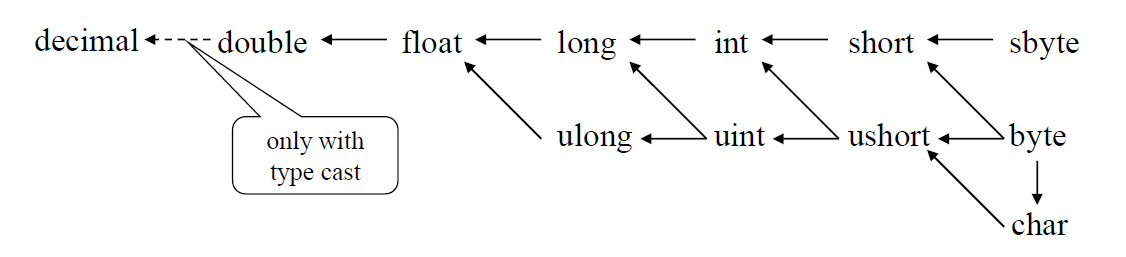
\includegraphics[width=\textwidth]{images/CSharp/TypenKompatibilitaet}
\end{minipage}
\hspace{0.1\textwidth}
\begin{minipage}{0.3\textwidth}
	folgende Beispiel sind gültig:
	\begin{lstlisting}
int var     = shortVar;
int var     = charVar;
float var   = charVar;
decimal var = (decimal)doubleVar;
	\end{lstlisting}
\end{minipage}



\subsubsection{Enumaration}
\begin{lstlisting}
	enum Color {Red, Blue, Green} // values: 0, 1, 2
	enum Access {Personal=1, Group=2, All=4}
	enum Access1 : byte {Personal=1, Group=2, All=4}
\end{lstlisting}

\subsubsection{Arrays}
Wie in in der Programiersprache C, beginnt der Index auch hier bei der Stelle 0.\\ \\
\textbf{One-dimensinal arrays}
\begin{lstlisting}
	int[] a = new int[3];
	int[] b = new int[] {3, 4, 5};
	int[] c = {3, 4, 5};
	SomeClass[] d = new SomeClass[10]; // array of references
	SomeStruct[] e = new SomeStruct[10]; // array of values (directly in the array)
\end{lstlisting}

\textbf{Multi-dimensional arrays (jagged)}\\
Hier können die Zeileneinträge verschieden lang sein, das heisst die Matrize ist nicht Rechteckig!
\begin{lstlisting}
	int[][] a = new int[2][]; // array of references to other arrays
	a[0] = new int[] {1, 2, 3}; // cannot be initialized directly
	a[1] = new int[] {4, 5};
	
	int x = a[0][1]; // x = 2
\end{lstlisting}

\textbf{Multi-dimensinal arrays (rectangular)}\\
Hier sind die Einträge in jeder Zeile gleich lang, dadurch wird die Matrize Rechteckig!
\begin{lstlisting}
	int[,] a = new int[2, 3]; // block matrix 
	int[,] b = {{1, 2, 3}, {4, 5, 6}}; // can be initialized directly 
	int[,,] c = new int[2, 4, 2];
	
	int x = a[0,1];
\end{lstlisting}

\textbf{Strings}
\begin{itemize}
	\item Können mit \textbf{+} verbunden werden z.B. \textit{''Don''} + s
	\item Können selektiert werden: z.B. s[i]
	\item Strings sind vom Type reference
	\item Können mit == und != verglichen werden
	\item Die String Länge kann mittels \textbf{s.Lenght()} ermittelt werden.
\end{itemize}

\subsubsection{Variable-length Array}
\begin{multicols}{2}

	\begin{lstlisting}
	using System;
	using System.Collections;
	class Test {
		static void Main() {
		ArrayList a = new ArrayList();
		a.Add("Charly");
		a.Add("Delta");
		a.Add("Alpha");
		a.Sort();
		for (int i = 0; i < a.Count; i++)
			Console.WriteLine(a[i]);
		}
	};
	\end{lstlisting}
	\columnbreak
	
	\textbf{Output}\\
		Alpha\\
		Charly\\
		Delta\\
\end{multicols}


\subsubsection{Associative Array}
\begin{multicols}{2}

	\begin{lstlisting}
	using System;
	using System.Collections;
	class Test {
		static void Main() {
		Hashtable phone = new Hashtable();
		phone["Karin"] = 7131;
		phone["Peter"] = 7130;
		phone["Wolfgang"] = 7132;
		foreach (string key in phone.Keys)
			Console.WriteLine("{0} = {1}", key, phone[key]);
		}
	};
	\end{lstlisting}
	\columnbreak
	
	\textbf{Output}\\
		Karin = 7131\\
		Peter = 7130\\
		Wolfgang = 7132\\
\end{multicols}


\subsubsection{Classes vs. Structs}
\setArrayStretch{1.5}
\begin{tabular}{|c|c|}
	\hline
    \textbf{Classes }&
    \textbf{Structs}\\
  \hline
	  Reference types (are allocated on the heap) &
	  Value types (are allocated on the stack)\\
  \hline
	  support inheritance &
	  no inheritance \\
	\hline
    can implement interfaces &
    can implement interfaces \\
  \hline
	  may declare a parameterless constructor & 
	  must not declare a parameterless constructor \\ 
	\hline
    may have a destructor &
    no destructor \\
  \hline
\end{tabular}

\subsubsection{System.Object}
System.Object ist die Basisklasse für alle Referenztypen.
\begin{lstlisting}
  object obj;
  obj = new Rectangle();  //obj kann Rectangle zugewiesen werden
  obj = new int[3];       //obj kann aber auch ein int array zugewiesen werden
\end{lstlisting}
  System.Object bietet noch weitere Funktionen an:
  \begin{itemize}
    \item  bool Equals(object o) $\rightarrow$ vergleicht zwei Objekte
    \item  string ToString() $\rightarrow$ gibt den Klassennamen als String aus
  \end{itemize}

\subsubsection{Boxing Unboxing}
\begin{figure}[h]
	\centering
	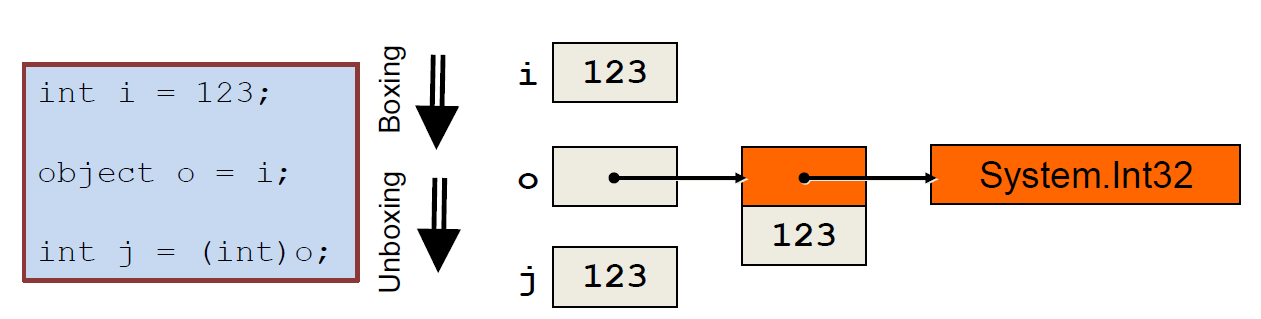
\includegraphics[height=3cm, ]{images/CSharp/BoxingUnboxing}
	\caption{Boxing Unboxing}	
\end{figure}

\textbf{Boxing}\\
Boxing ist wenn man eine Variable vom Stack auf den Heap legt. Das heisst man macht aus einer \textit{Value Type} einen \textit{Reference Type}.\\ 

\textbf{Unboxing}\\
Unboxing ist genau das Gegenteil. Hier holt man eine Variable vom Heap und legt sie auf den Stack. Das heisst man macht aus einem \textit{Reference Type} einen \textit{Value Type}.
